\documentclass[letterpaper,landscape]{article}
\usepackage{minitoc}
\usepackage{fullpage,enumitem,amsmath,amssymb,graphicx,algpseudocode,algorithm,array}
\usepackage{tikz}
\usepackage{mathtools}
\usepackage{minted}
\usepackage{multicol}
\usepackage{fancyhdr}
\usepackage{lastpage}
\usepackage{setspace}
\usepackage{titlesec}
\usepackage{enumitem}
\usepackage[margin=12pt,top=30pt,headsep=6pt,headheight=12pt]{geometry}
\usepackage[final]{pdfpages}

\setminted{fontsize=\footnotesize,
           frame=single,framesep=6pt,
           linenos,numbersep=6pt,xleftmargin=12pt,
           breaklines=true}
\usemintedstyle{colorful}

\pagestyle{fancy}
\fancyhf{}
\lhead{University of Minnesota - Is This A Class? - TRD 2022}
\rhead{\thepage/25}
\chead{\leftmark}

\titleformat{\section}{\normalfont\large\bfseries}{\thesection}{1em}{\setstretch{0.1}}
\titleformat{\subsection}{\normalfont\large\bfseries}{\thesubsection}{1em}{\setstretch{0.1}}

\parindent=0pt  % paragraphs DO NOT indent

\newcommand{\HSM}{\hskip .5em}
\newcommand{\DD}{\displaystyle}
\newcommand\invisiblesection[1]{%
  \refstepcounter{section}%
  \addcontentsline{toc}{section}{\protect\numberline{\thesection}#1}%
  \sectionmark{#1}}
\newcommand\invisiblesubsection[1]{%
  \refstepcounter{subsection}%
  \addcontentsline{toc}{subsection}{\protect\numberline{\thesubsection}#1}%
  \subsectionmark{#1}}

%\title{Stanford Cardinal '16 Notebook}
\begin{document}

\begingroup
\let\cleardoublepage\clearpage
\endgroup

\begin{multicols*}{3}

  %\raggedcolumns  

  \tableofcontents
%   \begin{enumerate}[label=\arabic*,leftmargin=*,labelsep=2ex,ref=\arabic*, nosep]
%     \setcounter{enumi}{9}
%     \setlist{nosep}
%       \begin{enumerate}[label*=.\arabic*,leftmargin=*,labelsep=2ex, nosep]
%         \itemsep 0em 
%         \item Geometric primitives \dotfill 21
%         \item Circles \dotfill 22
%         \item Polygons \dotfill 22
%         \item Misc. Point Set Problems \dotfill 23
%         \item 3D \dotfill 24
%       \end{enumerate}
%   \end{enumerate}

  \clearpage
  
  \section{Math}
    
    \subsection{Cramer's Rule}
    \[\begin{aligned}ax+by=e\\cx+dy=f\end{aligned}
    \Rightarrow
    \begin{aligned}x=\dfrac{ed-bf}{ad-bc}\\y=\dfrac{af-ec}{ad-bc}\end{aligned}\]
    
    In general, given an equation $Ax = b$, the solution to a variable $x_i$ is given by
    \[x_i = \frac{\det A_i'}{\det A} \]
    where $A_i'$ is $A$ with the $i$'th column replaced by $b$.
    
    \subsection{Trigonometry}
    \begin{align*}
    \sin(v+w)&{}=\sin v\cos w+\cos v\sin w\\
    \cos(v+w)&{}=\cos v\cos w-\sin v\sin w\\
    \tan(v+w)&{}=\dfrac{\tan v+\tan w}{1-\tan v\tan w}\\
    \sin v+\sin w&{}=2\sin\dfrac{v+w}{2}\cos\dfrac{v-w}{2}\\
    \cos v+\cos w&{}=2\cos\dfrac{v+w}{2}\cos\dfrac{v-w}{2}
    \end{align*}
    \[ (V+W)\tan(v-w)/2{}=(V-W)\tan(v+w)/2 \]
    where $V, W$ are lengths of sides opposite angles $v, w$.
    \begin{align*}
    	a\cos x+b\sin x&=r\cos(x-\phi)\\
    	a\sin x+b\cos x&=r\sin(x+\phi)
    \end{align*}
    where $r=\sqrt{a^2+b^2}, \phi=\operatorname{atan2}(b,a)$.
    
    \subsection{Triangles}
    Area: $A=\sqrt{s(s-a)(s-b)(s-c)}$\\
    Circumradius: $R=\dfrac{abc}{4A}$\\
    Inradius: $r=\dfrac{A}{s}$\\
    Length of median (divides triangle into two equal-area triangles): $m_a=\tfrac{1}{2}\sqrt{2b^2+2c^2-a^2}$\\
    Length of bisector (divides angles in two):\\ $s_a=\sqrt{bc\left[1-\left(\dfrac{a}{b+c}\right)^2\right]}$\\
    Law of sines: $\dfrac{\sin\alpha}{a}=\dfrac{\sin\beta}{b}=\dfrac{\sin\gamma}{c}=\dfrac{1}{2R}$\\
    Law of cosines: $a^2=b^2+c^2-2bc\cos\alpha$\\
    Law of tangents: $\dfrac{a+b}{a-b}=\dfrac{\tan\dfrac{\alpha+\beta}{2}}{\tan\dfrac{\alpha-\beta}{2}}$
    
    \subsection{Quadrilaterals}
    With side lengths $a,b,c,d$, diagonals $e, f$, diagonals angle $\theta$, area $A$ and
magic flux $F=b^2+d^2-a^2-c^2$:

\[ 4A = 2ef \cdot \sin\theta = F\tan\theta = \sqrt{4e^2f^2-F^2} \]

 For cyclic quadrilaterals the sum of opposite angles is $180^\circ$,
$ef = ac + bd$, and $A = \sqrt{(p-a)(p-b)(p-c)(p-d)}$.
    
    \subsection{Spherical coordinates}
    \begin{center}
    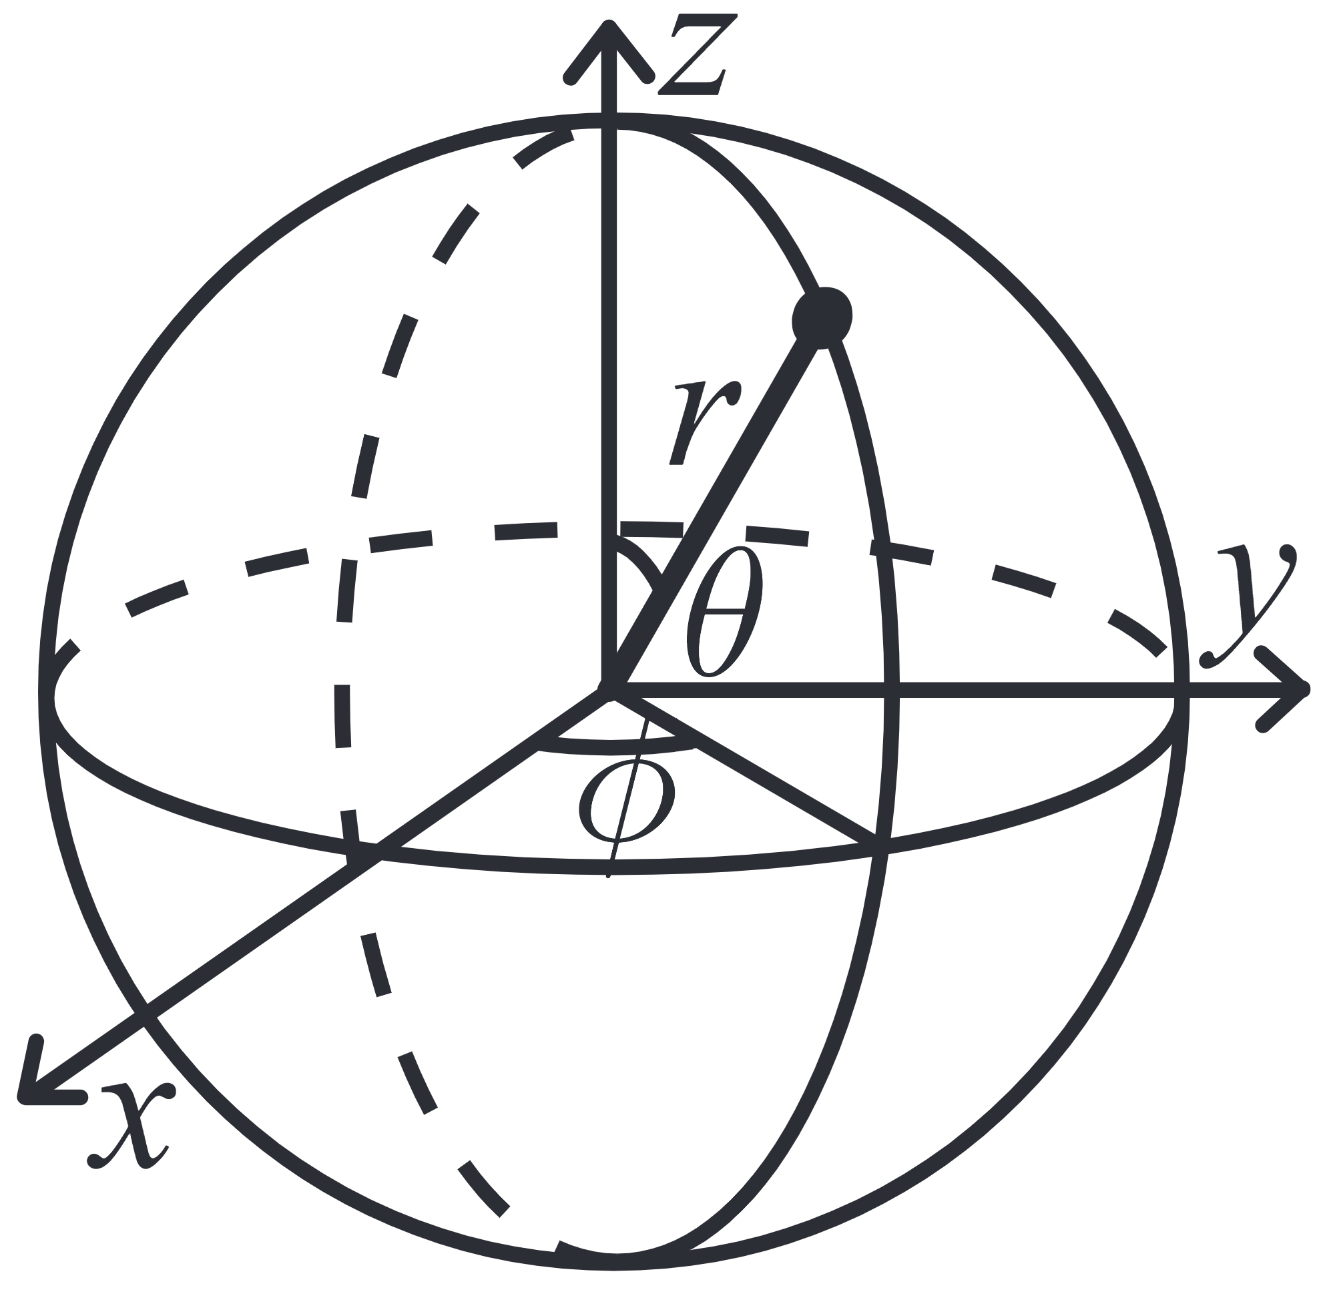
\includegraphics[width=25mm]{src/figures/SphericalCoordinates.png}
    \end{center}
    \[\begin{array}{cc}
    x = r\sin\theta\cos\phi & r = \sqrt{x^2+y^2+z^2}\\
    y = r\sin\theta\sin\phi & \theta = \textrm{acos}(z/\sqrt{x^2+y^2+z^2})\\
    z = r\cos\theta & \phi = \textrm{atan2}(y,x)
    \end{array}\]

  
    \subsection{Sums \& Combinatorics}
  
    $\sum_{k=0}^{n}k=n(n+1)/2$\\
    $\sum_{k=0}^{n}k^{2}=n(n+1)(2n+1)/6$\\
    $\sum_{k=0}^{n}k^{3}=n^{2}(n+1)^{2}/4$\\
    $\sum_{k=0}^{n}k^{4}=(6n^{5}+15n^{4}+10n^{3}-n)/30$\\
    $\sum_{k=0}^{n}k^{5}=(2n^{6}+6n^{5}+5n^{4}-n^{2})/12$\\
    $\sum_{k=0}^{n}x^{k}=(x^{n+1}-1)/(x-1)$\\
    $\sum_{k=0}^{n}kx^{k}=(x-(n+1)x^{n+1}+nx^{n+2})/(x-1)^{2}$\\
    ${n \choose k}=\frac{n!}{(n-k)!k!}$\\
    ${n \choose k}={n-1 \choose k}+{n-1 \choose k-1}$\\
    ${n \choose k}=\frac{n}{n-k}{n-1 \choose k}$\\
    ${n \choose k}=\frac{n-k+1}{k}{n \choose k-1}$\\
    ${n+1 \choose k}=\frac{n+1}{n-k+1}{n \choose k}$\\
    ${n \choose k+1}=\frac{n-k}{k+1}{n \choose k}$\\
    $\sum_{k=1}^{n}k\tbinom{n}{k}=n2^{n-1}$\\
    $\sum_{k=1}^{n}k^{2}\tbinom{n}{k}=(n+n^{2})2^{n-2}$\\
    ${m+n \choose r}=\sum_{k=0}^{r}{m \choose k}{n \choose r-k}$\\
    ${n \choose k}=\prod_{i=1}^{k}\frac{n-k+i}{i}$\\
    \textbf{Hockey stick Formulas:}\\
    $\sum_{i=k}^n {i \choose k} = {n+1 \choose k+1}$\\
    ${n+1 \choose n-k} = \sum_{j=0}^{n-k} {j+k \choose k} = \sum_{j=0}^{n-k} {j+k \choose j}$\\
    \textbf{Taylor Series:}\\
    $f(x) = \sum_{n=0}^\infty \frac{f^{(n)}(a)}{n!}(x-a)^n$
  
    \subsection{Burnside's Lemma}
    Given a group $G$ of symmetries and a set $X$, the number of elements of $X$ \emph{up to symmetry} equals
		 \[ {\frac {1}{|G|}}\sum _{{g\in G}}|X^{g}|, \]
		 where $X^{g}$ are the elements fixed by $g$ ($g.x = x$).

		 If $f(n)$ counts ``configurations'' (of some sort) of length $n$, we can ignore rotational symmetry using $G = \mathbb Z_n$ to get
		 \[ g(n) = \frac 1 n \sum_{k=0}^{n-1}{f(\text{gcd}(n, k))} = \frac 1 n \sum_{k|n}{f(k)\phi(n/k)}. \]
    \subsection{Distributions}

    \subsubsection{Binomial distribution}
    The number of successes in $n$ independent yes/no experiments, each which yields success with probability $p$ is $\textrm{Bin}(n,p),\,n=1,2,\dots,\, 0\leq p\leq1$.
    \[p(k)=\binom{n}{k}p^k(1-p)^{n-k}\]
    \[\mu = np,\,\sigma^2=np(1-p)\]
    $\textrm{Bin}(n,p)$ is approximately $\textrm{Po}(np)$ for small $p$.
    
    \subsubsection{First success distribution}
    The number of trials needed to get the first success in independent yes/no experiments, each wich yields success with probability $p$ is $\textrm{Fs}(p),\,0\leq p\leq1$.
    \[p(k)=p(1-p)^{k-1},\,k=1,2,\dots\]
    \[\mu = \frac1p,\,\sigma^2=\frac{1-p}{p^2}\]
    
    \subsubsection{Poisson distribution}
    The number of events occurring in a fixed period of time $t$ if these events occur with a known average rate $\kappa$ and independently of the time since the last event is $\textrm{Po}(\lambda),\,\lambda=t\kappa$.
    \[p(k)=e^{-\lambda}\frac{\lambda^k}{k!}, k=0,1,2,\dots\]
    \[\mu=\lambda,\,\sigma^2=\lambda\]
    
    \subsubsection{Normal distribution}
    Most real random values with mean $\mu$ and variance $\sigma^2$ are well described by $\mathcal{N}(\mu,\sigma^2),\,\sigma>0$.
    \[ f(x) = \frac{1}{\sqrt{2\pi\sigma^2}}e^{-\frac{(x-\mu)^2}{2\sigma^2}} \]
    If $X_1 \sim \mathcal{N}(\mu_1,\sigma_1^2)$ and $X_2 \sim \mathcal{N}(\mu_2,\sigma_2^2)$ then
    \[ aX_1 + bX_2 + c \sim \mathcal{N}(\mu_1+\mu_2+c,a^2\sigma_1^2+b^2\sigma_2^2) \]
    
    \subsection{Primes}
    \textbf{Lucas' Theorem:} For non-negative integers $m$ and $n$ and a prime $p$,
     
     $$\binom{m}{n}\equiv\prod_{i=0}^k\binom{m_i}{n_i}\pmod p,$$
    where
    $$m=m_kp^k+m_{k-1}p^{k-1}+\cdots +m_1p+m_0$$
    is the base $p$ representation of $m$, and similarly for $n$.
  
    \textbf{Prime Number Theorem:} $\pi(x) \approx \frac{x}{\ln(x)}$ is the \# of primes $\leq x$.\\
    \resizebox{26.5 em}{!}{
            \begin{tabular}{c|c}
                $n$& $\pi(10^n)$\\ \hline
                1  & 4\\
                2  & 25\\
                3  & 168\\
                4  & 1,229\\
                5  & 9,592\\
                6  & 78,498\\
                7  & 664,579\\
                8  & 5,761,455\\
                9  & 50,847,534\\
                10 & 455,052,511\\
                11 & 4,118,054,813\\
                12 & 37,607,912,018
            \end{tabular}
            \begin{tabular}{c | c}
                13 & 346,065,536,839\\
                14 & 3,204,941,750,802\\
                15 & 29,844,570,422,669\\
                16 & 279,238,341,033,925\\
                17 & 2,623,557,157,654,233\\
                18 & 24,739,954,287,740,860\\
                19 & 234,057,667,276,344,607\\
                20 & 2,220,819,602,560,918,840\\
                21 & 21,127,269,486,018,731,928\\
                22 & 201,467,286,689,315,906,290\\
                23 & 1,925,320,391,606,803,968,923\\
                24 & 18,435,599,767,349,200,867,866\\
                25 & 176,846,309,399,143,769,411,680
            \end{tabular}
        }
    
    \subsection{Stirling Numbers of the second kind}
    Number of ways to partition a set of $n$ numbers into $k$ non-empty subsets.
    
    $${n \brace k}=\frac{1}{k!}\sum_{j=0}^{k}(-1)^{(k-j)}{k \choose j}j^n$$
    $${0 \brace 0}=1, \hskip 5em {n \brace 0}={0 \brace n}=1$$
    $${n+1 \brace k}=k{n \brace k}+{n \brace k-1}$$
      
    \subsection{Derangements}
	Permutations of a set such that none of the elements appear in their original position.\\
	$\mkern-2mu D(n) = (n-1)(D(n-1)+D(n-2))$\\ $\DD \hskip 100em = n D(n-1)+(-1)^n = \left\lfloor\frac{n!}{e}\right\rceil$
	
	\subsection{Partition function}
	Number of ways of writing $n$ as a sum of positive integers, disregarding the order of the summands.
	\[ p(0) = 1,\ p(n) = \sum_{k \in \mathbb Z \setminus \{0\}}{(-1)^{k+1} p(n - k(3k-1) / 2)} \]
	\[ p(n) \sim 0.145 / n \cdot \exp(2.56 \sqrt{n}) \]

	\begin{center}
    	\begin{tabular}{c|c@{\ }c@{\ }c@{\ }c@{\ }c@{\ }c@{\ }c@{\ }c@{\ }c@{\ }c@{\ }c@{\ }c@{\ }c}
    		$n$    & 0 & 1 & 2 & 3 & 4 & 5 & 6  & 7  & 8  & 9  & 20  & 50  & 100 \\ \hline
    		$p(n)$ & 1 & 1 & 2 & 3 & 5 & 7 & 11 & 15 & 22 & 30 & 627 & $\mathtt{\sim}$2e5 & $\mathtt{\sim}$2e8 \\
    	\end{tabular}
	\end{center}
	
	\subsection{Bell numbers}
	Total number of partitions of $n$ distinct elements. $B(n) =$
	$1, 1, 2, 5, 15, 52, 203, 877, 4140, 21147, \dots$. For $p$ prime,
	\[ B(p^m+n)\equiv mB(n)+B(n+1) \pmod{p} \]
	
	\subsection{Catalan numbers}
	\[ C_n=\frac{1}{n+1}\binom{2n}{n}= \binom{2n}{n}-\binom{2n}{n+1} = \frac{(2n)!}{(n+1)!n!} \]
	\[ C_0=1,\ C_{n+1} = \frac{2(2n+1)}{n+2}C_n,\ C_{n+1}=\sum C_iC_{n-i} \]
	${C_n = 1, 1, 2, 5, 14, 42, 132, 429, 1430, 4862, 16796, 58786, \dots}$
	\begin{itemize}[noitemsep]
		\item sub-diagonal monotone paths in an $n\times n$ grid.
		\item strings with $n$ pairs of parenthesis, correctly nested.
		\item binary trees with with $n+1$ leaves (0 or 2 children).
		\item ordered trees with $n+1$ vertices.
		\item ways a convex polygon with $n+2$ sides can be cut into triangles by connecting vertices with straight lines.
		\item permutations of $[n]$ with no 3-term increasing subseq.
	\end{itemize}
	
	\subsection{Erd\H{o}s--Gallai theorem}
	A simple graph with node degrees $d_1 \geq \dots \geq d_n$ exists iff 
	$d_1 + \dots + d_n$ is even, and for every $k = 1 \dots n$:\\
	$$\DD \sum_{i=1}^k d_i \leq k(k-1) + \sum_{i=k+1}^n \min(d_i, k)$$
	
	\subsection{Misc}
	 \textbf{Bayes' Theorem:} $P(A | B) = \frac{P(B | A) P(A)}{P(B)}$\\
	 \textbf{Planar Graph Formula:} $v - e + f = 2$
	 
    \section{CPP Header, Compilation}
    \inputminted{cpp}{src/header.h}
\end{multicols*}  
  
\begin{multicols*}{2}
  \section{String Algorithms}
  \subsection{Aho Corasick}
  \inputminted{java}{src/Strings/AhoCorasick.java}
  
  \subsection{Prefix, Z, and Manacher Functions}
  \inputminted{java}{src/Strings/Strings.java}
  
  \subsection{Suffix Array}
  \inputminted{java}{src/Strings/SuffixArray.java}
  
  \section{Data structures}
  
  \subsection{Disjoint Set}
  \inputminted{java}{src/DS/DisjointSet.java}
  
  \subsection{Segment Tree}
  \inputminted{java}{src/DS/SegmentTree.java}
  \inputminted{cpp}{src/DS/SegmentTree.cpp}
  
  \subsection{Lazy Segment Tree}
  \inputminted{cpp}{src/DS/LazySegTree.cpp}
  
  \subsection{Fenwick Tree}
  \inputminted{cpp}{src/DS/FenwickTree.cpp}
  
  \subsection{Order Statistic Tree}
  \inputminted{cpp}{src/DS/OrderStatisticTree.cpp}
  
  
  \section{Graph Algorithms}
  
  \subsection{Dinics Max Flow}
  \inputminted{java}{src/Graphs/DinicsMaxFlow.java}
  
  \subsection{Min Cost Flow}
  \inputminted{java}{src/Graphs/MinCostFlow.java}
  
  \subsection{Euler Walk}
  \inputminted{java}{src/Graphs/EulerWalk.java}
  
  \subsection{Bellman Ford}
  \inputminted{java}{src/Graphs/BellmanFord.java}
  
  \subsection{Floyd Warshall}
  \inputminted{java}{src/Graphs/FloydWarshall.java}
  
  \subsection{Strongly Connected Components}
  \inputminted{java}{src/Graphs/SCComponents.java}
  
  \subsection{Segment Tree LCA}
  \inputminted{java}{src/Graphs/SegmentLCA.java}
  
  \subsection{Binary Lifting LCA}
  \inputminted{cpp}{src/Graphs/BinaryLiftingLCA.cpp}
  
  \subsection{Bipartite Maximum Matching}
  \inputminted{cpp}{src/Graphs/BipartiteMaximumMatching.cpp}
  
  \subsection{Erdos-Gallai}
  \inputminted{cpp}{src/Graphs/ErdosGallai.cpp}
  
  \section{Number Theory}
  
  \subsection{CRT, GCD, LCM, Inverse, Pow, SQRT}
  \inputminted{java}{src/Number_Theory/NumberTheory.java}
  
  \subsection{Primes}
  \inputminted{java}{src/Number_Theory/Prime.java}
  
  
  \section{Linear Algebra}
  
  \subsection{Matrix Multipliaction}
  \inputminted{cpp}{src/LinAlg/MatMultiply.cpp}
    
  \subsection{Inverse and Determinant}
  \inputminted{cpp}{src/LinAlg/GaussJordan.cpp}
  
  \subsection{Modular RREF}
  \inputminted{cpp}{src/LinAlg/ModularRREF.cpp}
  
  \subsection{RREF}
  \inputminted{cpp}{src/LinAlg/RREF.cpp}
  
  
  \section{Misc}
  \subsection{Bit Tricks}
  \inputminted{cpp}{src/Misc/BitTricks.cpp}
  
  \subsection{CPP Builtins}
  \inputminted{text}{src/Misc/CPPBuiltins.cpp}
  
  \subsection{CPP Syntax Examples}
  \inputminted{cpp}{src/Misc/CPPSyntaxExamples.cpp}
  
  \subsection{Bisect \& Ternary Search}
  \inputminted{java}{src/Misc/Bisect.java}
  
  \subsection{Knapsack}
  \inputminted{java}{src/Misc/Knapsack.java}
  
  \subsection{Longest Increasing Subsequence}
  \inputminted{java}{src/Misc/LIS.java}
  
  \subsection{Fast Fourier Transform}
  \inputminted{cpp}{src/Misc/FFT.cpp}
  
  \subsection{Polynomial Interpolation}
  Description: Given $n$ points (x[i], y[i]), computes an n-1-degree polynomial $p$ that passes through them: $p(x) = a[0]*x^0 + ... + a[n-1]*x^{n-1}$. For numerical precision, pick $x[k] = c*\cos(k/(n-1)*\pi), k=0 \dots n-1$.
  \inputminted{cpp}{src/Misc/PolyInterpolate.cpp}
  
  \subsection{Dates}
  \inputminted{cpp}{src/Misc/Dates.cpp}
  
  \subsection{Java Templates}
  \inputminted{java}{src/Misc/JavaTricks.java}
  

  
\end{multicols*}

\invisiblesection{Geometry}
\invisiblesubsection{Geometric primitives}

\includepdf[pages={19},pagecommand={},width=1.05\textwidth]{kactlColored.pdf}
\invisiblesubsection{Circles}
\invisiblesubsection{Polygons}

\includepdf[pages={20},pagecommand={},width=1.05\textwidth]{kactlColored.pdf}
\invisiblesubsection{Misc. Point Set Problems}

\includepdf[pages={21},pagecommand={},width=1.05\textwidth]{kactlColored.pdf}
\invisiblesubsection{3D}

\includepdf[pages={22},pagecommand={},width=1.05\textwidth]{kactlColored.pdf}

\let\clearpage\relax
\end{document}


